\documentclass[12pt]{article}

\usepackage{graphicx}
\usepackage{pdfpages}
\usepackage{listings}
\usepackage{amsmath}
\usepackage{subcaption}
\usepackage{todonotes}
\usepackage{arydshln}

\renewcommand{\figurename}{Fig.}

\title{TTK4210 Advanced Control of Industrial Systems, Exercise 6}
\date{}
\author{Kristian Løvland}

\begin{document}
\maketitle
\tableofcontents

\newpage
\section{Abstract}
In this project, a model of a butane distillation column was used to design a controller for the composition of two product streams consisting of n-butane and iso-butane, respectively. By identifying characteristics of relevant subsystems, PI controllers for the states of these systems were designed with the ultimate goal of keeping the purity of the products at a satisfactory level.

\newpage
\section{Introduction}
The stream of control engineers is flowing slower than before, but still steadily into lucrative jobs in the process industry. As a part of this, all children learn about hydrocarbon chains in middle school, and every cybernetics student at NTNU learns how to control plants that are common in the petroleum industry. This report is simply me doing my part.

A good introduction to the control problem we're faced with is given in the assignment text \todo{Legg til kilde}. A short summary of this follows here.

Our final goal is to have a control system giving two product flows out of the distillation column having the desired compositions $x_D^*$ and $x_B^*$. In practice, we control our compositions $x_D$ and $x_B$ indirectly through the temperatures in the locations of the product streams, denoted $T_D$ and $T_B$.

To achieve this, some more control is needed. The levels $M_D$ and in the top accumulator and $M_B$ in the destillation column needs to be controlled to stable setpoints. The same goes for distillation column pressure $p$.

To control these five variables, five degrees of freedom is needed. These are all flow rates, denoted $V_T$, $L$, $D$, $V$, $B$. Each of these is controlled more or less directly by a valve.

Independent control of all of the variables are used. Table \ref{tab:pairings} shows the pairing of manipulated and controlled variables. It is assumed that choosing godd setpoints for $T_D$ and $T_B$ gives satisfactory product quality. The control structure used here is called LV-control, after the manipulated variables used to (indirectly) control product quality.

\begin{table}[h]
\centering
\begin{tabular}{c|c}
Manipulated variable & Controlled variable \\ \hline
$V_T$ & $p$ \\
$D$ & $M_D$ \\
$B$ & $M_B$ \\
$L$ & $T_D$ \\
$V$ & $T_B$
\end{tabular}
\caption{Variable pairings}
\label{tab_pairings}
\end{table}

\subsection{A few words on scaling}
The scaling and units used in this report might seem a bit arbitrary. Despite how it might seem, I have tried to be consistent. For my own sake, all plots of variables are in engineering units, the same goes for all controller gains $K_p$. These have been converted to internally scaled gain when implementing the controllers in K-spice. Units (or the lack of them) for plots used in frequency analysis and loop-shaping are hopefully unambiguous.

\newpage
\section{Tuning secondary controllers}
The secondary controllers were tuned individually using the SIMC method for PI controllers. A step in process input with an amplitude small enough to not cause problems (usually meaning 50\% of maximum accepted input magnitude) in other parts of the system was used for all the secondary controllers, controlling the states $D$, $L$, $B$, $V$ and $p$.

In short, the SIMC tuning method can be summarized as follows (using notation from \cite{regtek}) \todo{Legg til kilde, regtekboka}

\begin{enumerate}
\item Fit the step response to a first order model. This means finding time delay $\tau$, slope $k' = \frac{dy/dt}{\Delta u}$ and time constant $T_1$ from the plot of the step response.
\item To achieve the desired time constant $T_L$, use the PI controller parameters $K_p = \frac{1}{k'} \frac{1}{\tau + T_L}$, $T_i = \min(T_1, 4(\tau + T_L))$.
\end{enumerate}

% Figurer, open-loop stegrespons
\begin{figure}
\centering
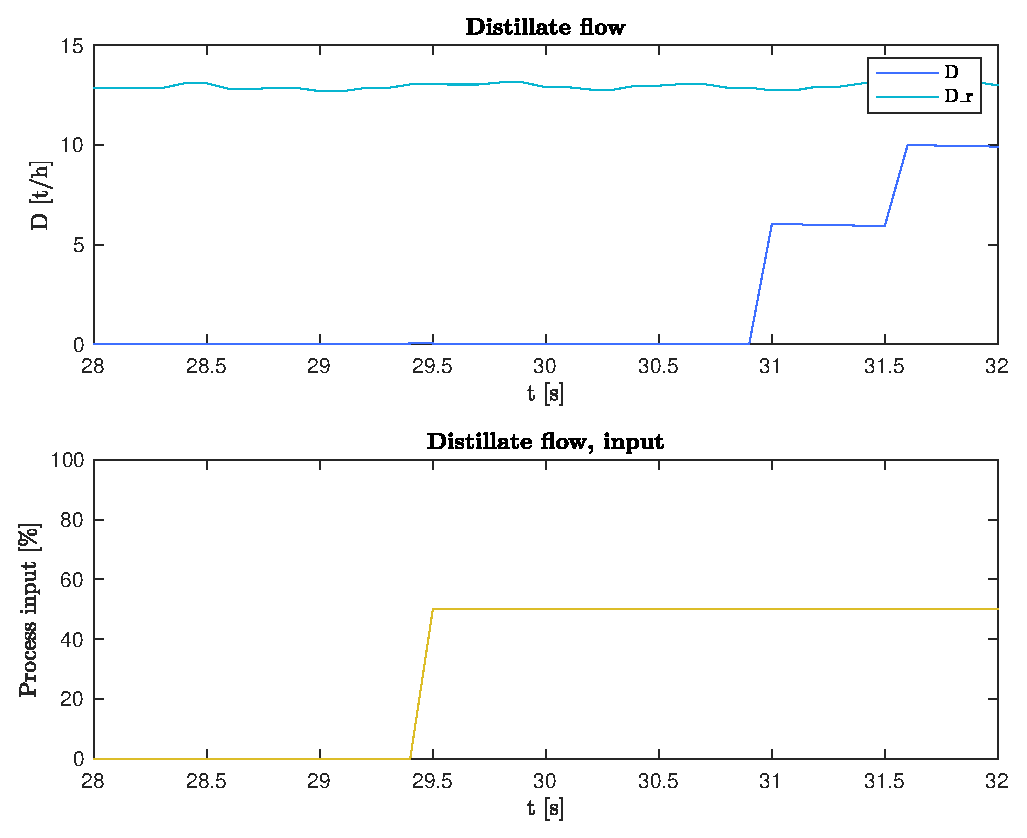
\includegraphics[width=0.8\textwidth]{../Systemanalyse/Log_Data_to_Matlab/Figurer/Stegeksperimenter/FC1005.eps}
\caption{Open-loop step response of $D$}
\label{fig:ol_step_FC1005}

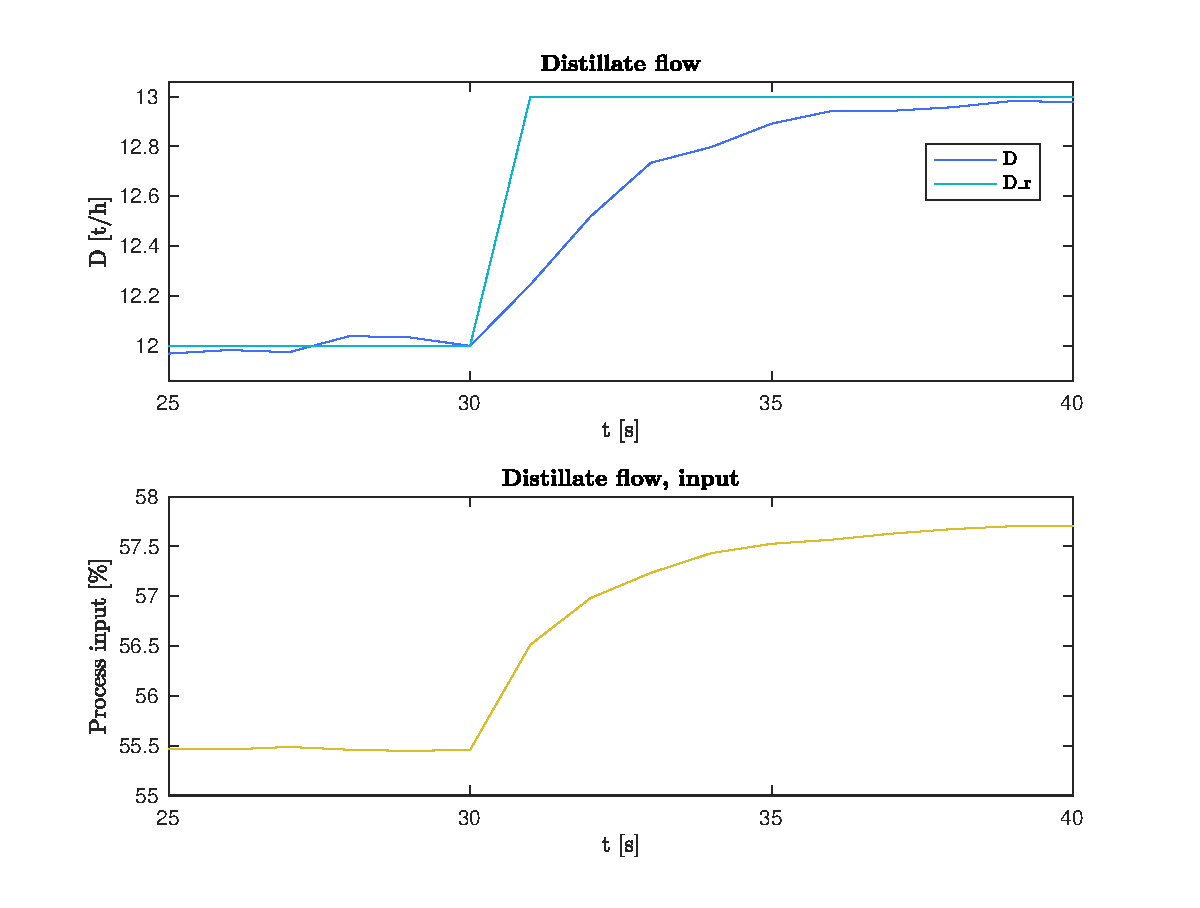
\includegraphics[width=0.8\textwidth]{../Systemanalyse/Log_Data_to_Matlab/Figurer/Stegeksperimenter/FC1005_step.eps}
\caption{Closed-loop step response of $D$}
\label{fig:cl_step_FC1005}
\end{figure}

\begin{figure}
\centering
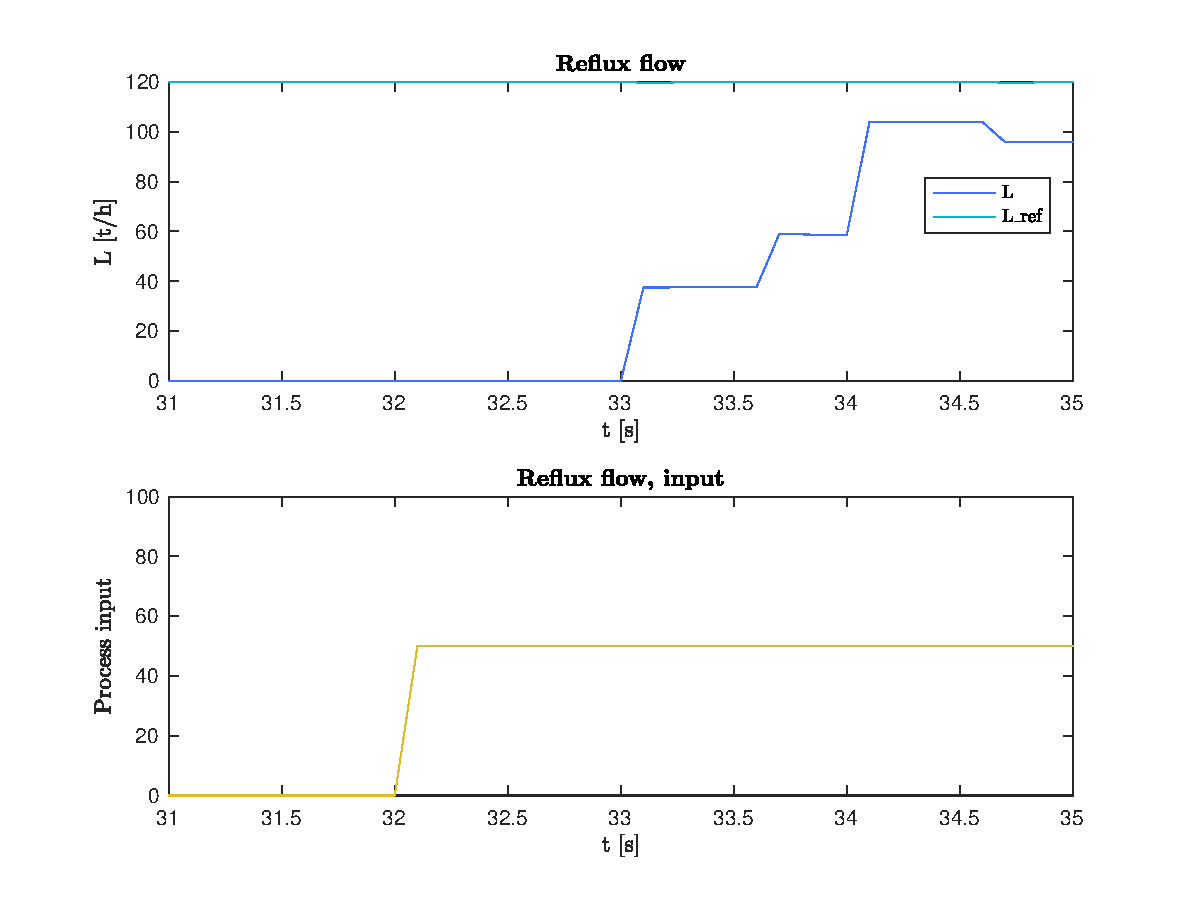
\includegraphics[width=0.8\textwidth]{../Systemanalyse/Log_Data_to_Matlab/Figurer/Stegeksperimenter/FC1015.eps}
\caption{Open-loop step response of $L$}
\label{fig:ol_step_FC1015}

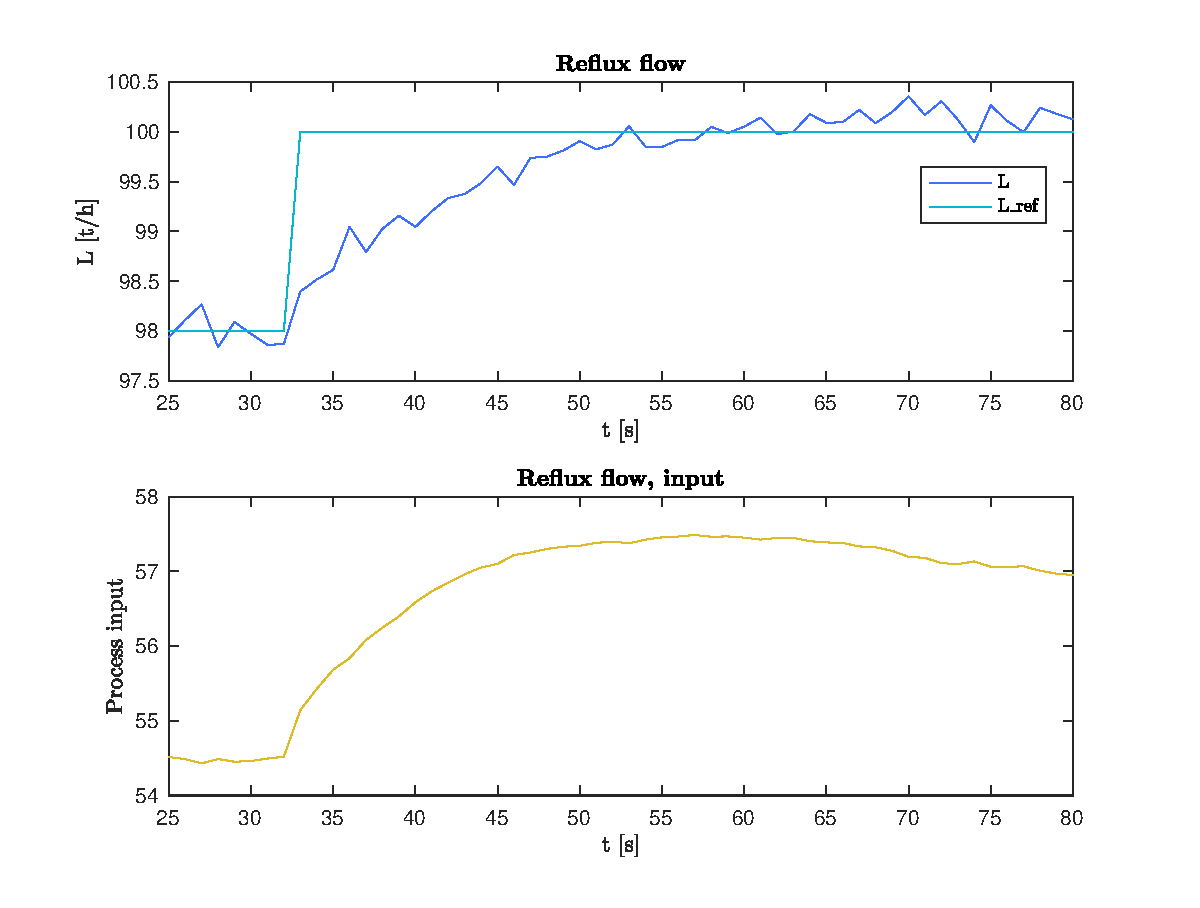
\includegraphics[width=0.8\textwidth]{../Systemanalyse/Log_Data_to_Matlab/Figurer/Stegeksperimenter/FC1015_step.eps}
\caption{Closed-loop step response of $L$}
\label{fig:cl_step_FC1015}
\end{figure}

\begin{figure}
\centering
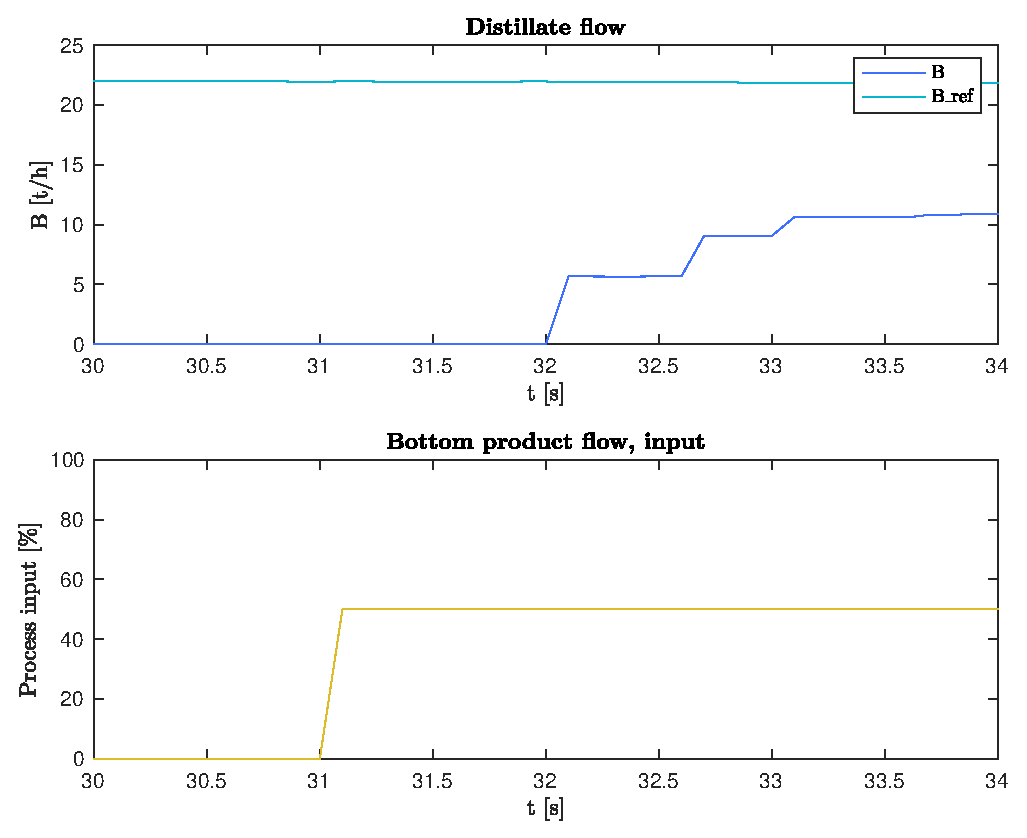
\includegraphics[width=0.8\textwidth]{../Systemanalyse/Log_Data_to_Matlab/Figurer/Stegeksperimenter/FC1019.eps}
\caption{Open-loop step response of $B$}
\label{fig:ol_step_FC1019}

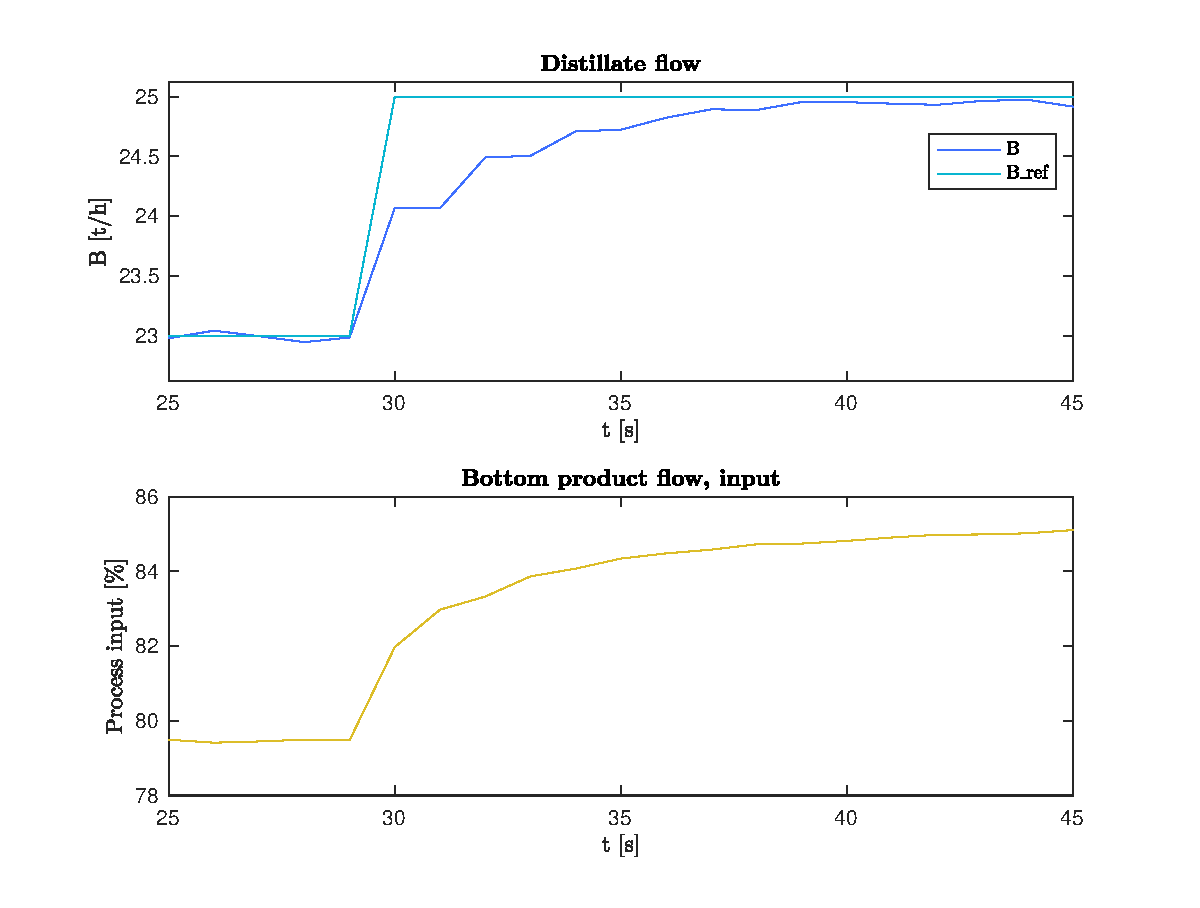
\includegraphics[width=0.8\textwidth]{../Systemanalyse/Log_Data_to_Matlab/Figurer/Stegeksperimenter/FC1019_step.eps}
\caption{Closed-loop step response of $B$}
\label{fig:cl_step_FC1019}
\end{figure}

\begin{figure}
\centering
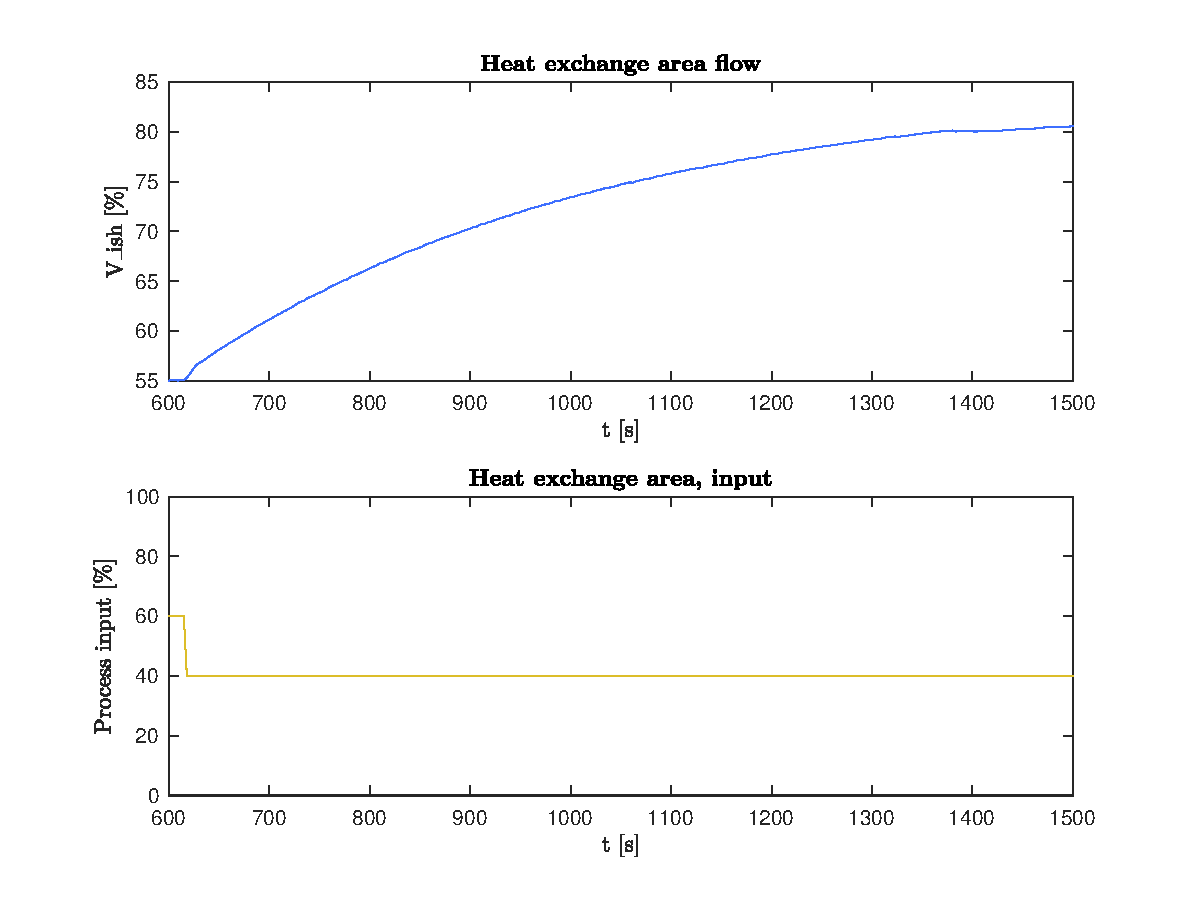
\includegraphics[width=0.8\textwidth]{../Systemanalyse/Log_Data_to_Matlab/Figurer/Stegeksperimenter/LC1028.eps}
\caption{Open-loop step response of heat exchanger area, related to $V$}
\label{fig:ol_step_LC1028}

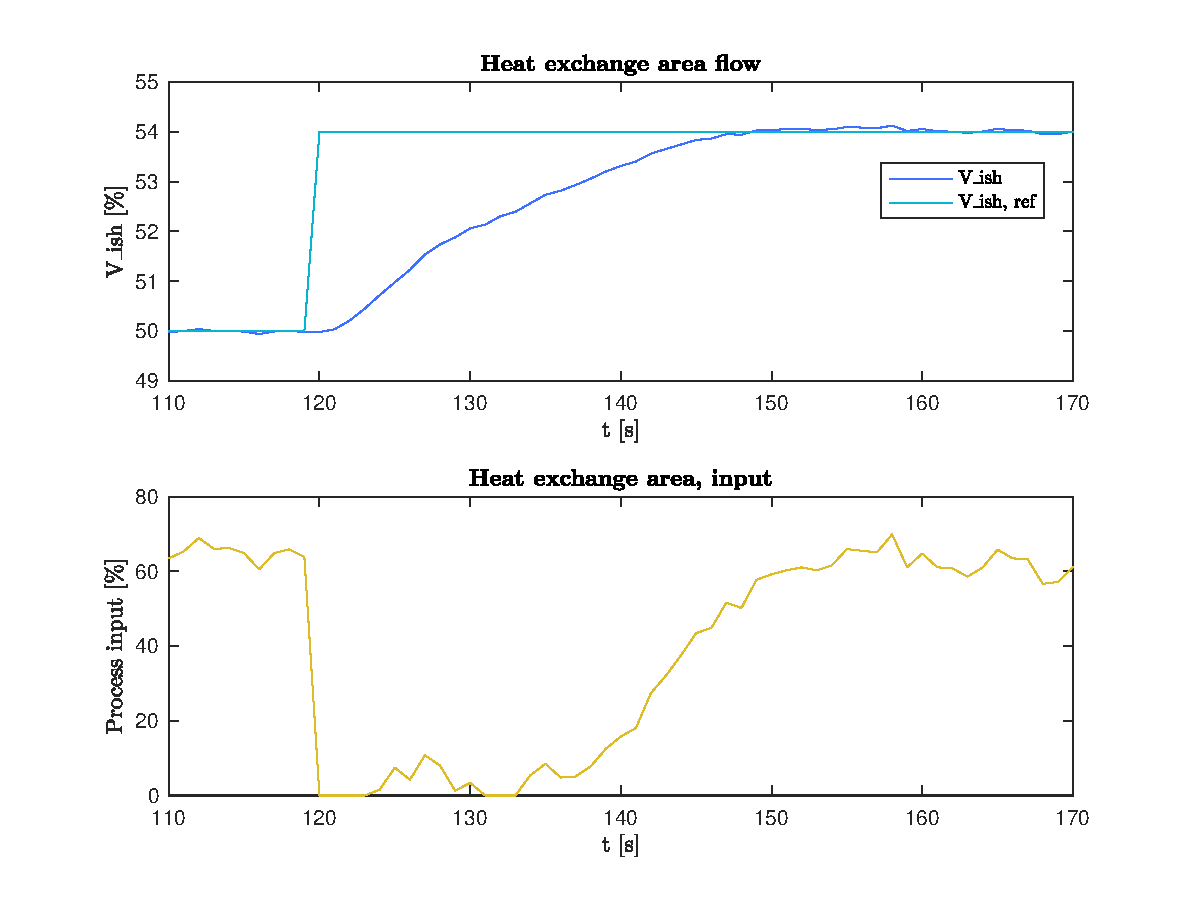
\includegraphics[width=0.8\textwidth]{../Systemanalyse/Log_Data_to_Matlab/Figurer/Stegeksperimenter/LC1028_step.eps}
\caption{Closed-loop step response of heat exchanger area, related to $V$}
\label{fig:cl_step_LC1028}
\end{figure}

\begin{figure}
\centering
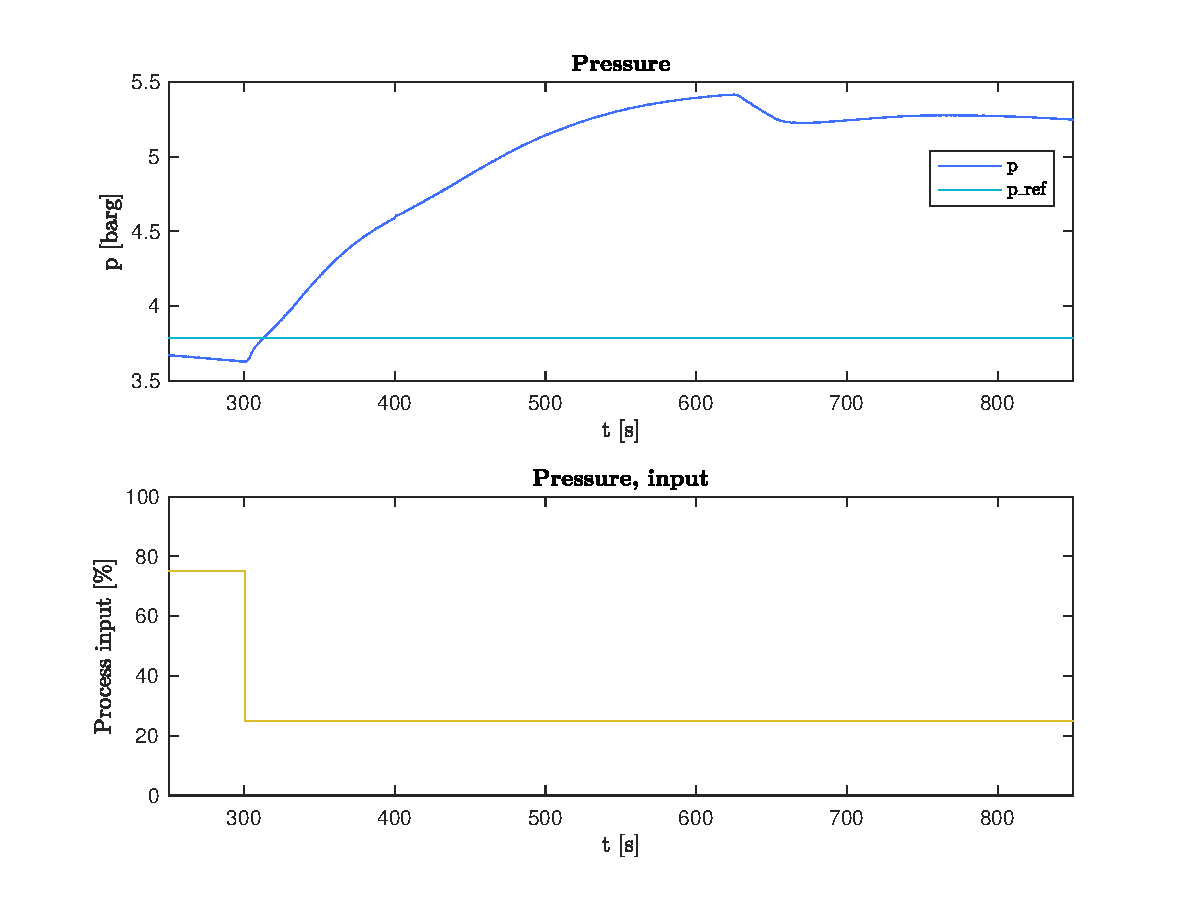
\includegraphics[width=0.8\textwidth]{../Systemanalyse/Log_Data_to_Matlab/Figurer/Stegeksperimenter/PC1024.eps}
\caption{Open-loop step response of $p$}
\label{fig:ol_step_PC1024}

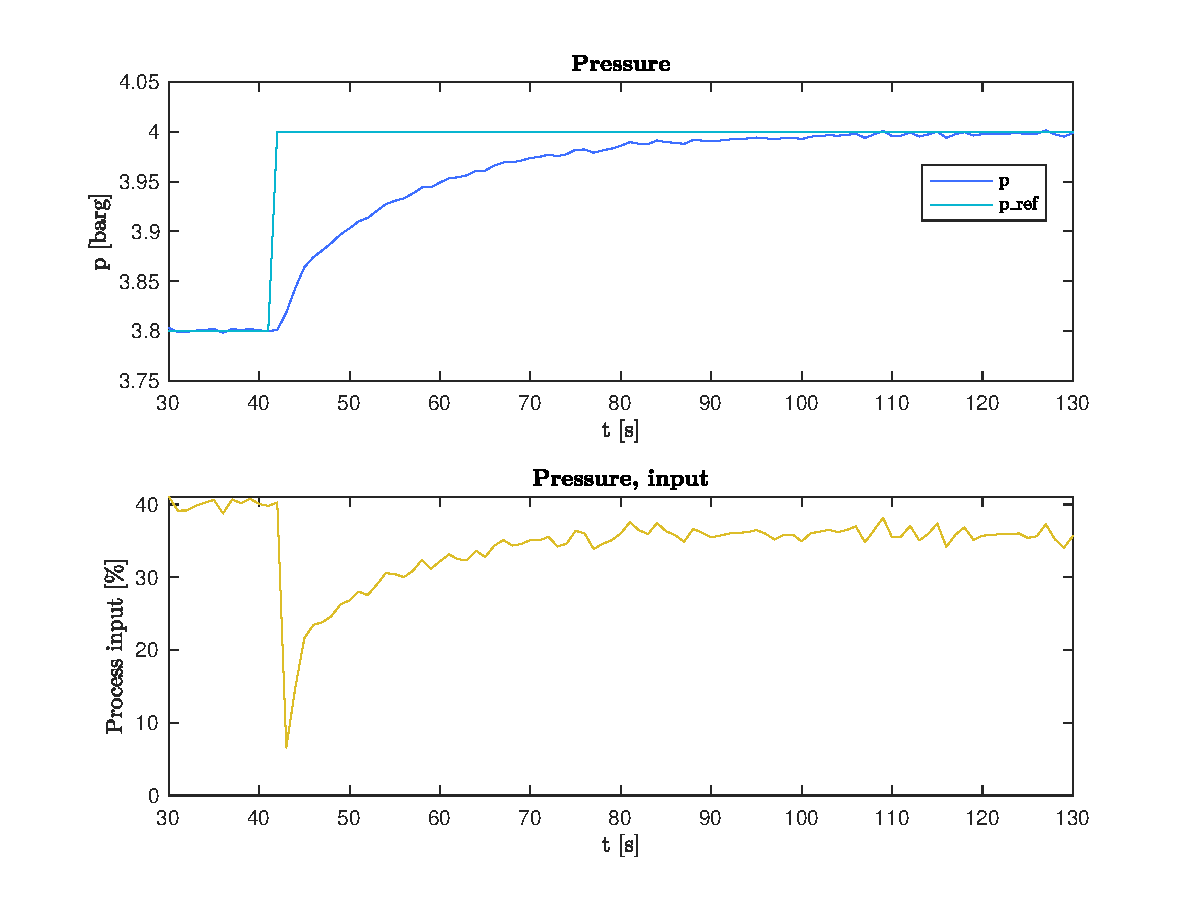
\includegraphics[width=0.8\textwidth]{../Systemanalyse/Log_Data_to_Matlab/Figurer/Stegeksperimenter/PC1024_step.eps}
\caption{Closed-loop step response of $p$}
\label{fig:cl_step_PC1024}
\end{figure}

The data from these experiments can be seen in figures \ref{fig:ol_step_FC1005}, \ref{fig:ol_step_FC1015}, \ref{fig:ol_step_FC1019}, \ref{fig:ol_step_LC1028} and \ref{fig:ol_step_PC1024}. The reference signals should have been omitted from these plots since we are dealing with open loop systems, and can safely be ignored here.

The plots show that for the first three variables, the accuracies of the simulations are clearly not sufficient for fitting a first order model (they behave in a stepwise fashion). Inspecting the order of magnitude of the gains and time constants is, however, still useful. An attempt at making sense of these parameters is shown in table \ref{tab:inner_loop_step_responses}, together with the fitted values for $V$ and $p$.

Simple linear fitting from initial to steady-state value was used for the three quick states, which gives conservative estimates of $k'$ and $T_1$. In the table, a desired time constant for the controlled system $T_L$ is shown in the rightmost column. For a quick response, choosing $T_L = 0,3\tau$ is suggested in \cite{balchen}. Some simple trial and error in K-spice showed that this lead to oscillation and unfortunate interaction between control loops, especially the controllers for $D$ and $L$. This is probably partly due to the underestimates of $k'$ and $T_1$ for these variables, since conservative estimates of these results in more aggressive controllers (to compensate for the slow system) when using the SIMC method.

Due to this unsatisfactory behaviour, $T_L = 2\tau$ was chosen for the three fastest control loops instead. The time delay was hard to make a meaningful reading of for the two other systems, so a somewhat arbitrary choice of $T_L = 10s$ was chosen for these systems (instead of using the $T_L = 2\tau$ rule). Like all the other parameters, these were not absolute choices, but a good starting point for further tuning.

After calculating the SIMC controller values some qualitative tuning using K-spice simulations was, not surprisingly, needed. For $D$ and $L$, the integral times were kept fixed, and the gain was decreased to avoid oscillations. For $B$, it was necessary to reduce the integral time in addition to reducing the gain, to avoid oscillation. The response of $V$ was slow, and to avoid bandwith limitations in the control of $T_B$ later, both controller parameters were changed to give dramatically more aggressive behaviour. For $p$, the stationary deviation was removed a bit slowly, so the integral time was reduced, while also reducing gain to avoid oscillation.


The results of implementing these controllers in K-spice, using the internally scaled gain $G = K_p \frac{(y_{\max} - y_{\min})}{(u_{\max} - u_{\min})}$ for all controllers, are shown in figures \ref{fig:cl_step_FC1005}, \ref{fig:cl_step_FC1015}, \ref{fig:cl_step_FC1019}, \ref{fig:cl_step_LC1028} and \ref{fig:cl_step_PC1024}.


\begin{table}
\centering
\begin{tabular}{c | c | c | c | c | c || c}
& $\tau$ & $T_1$ & $\frac{dy}{dt}$ & $\Delta u$ & $k'$ & $T_L$ \\ \hline
$D$ & 1,0s & 0,4s & 14,3 & 50\% & 28,6 & 2s \\
$L$ & 1,0s & 1,0s & 47,5 & 50\% & 95,0 & 2s \\
$B$ & 1,0s & 0,6s & 10,0 & 50\% & 20,0 & 2s \\
$V$ & $\approx$ 0 & 400s & 0,028 & 20\% & 0,14 & 10s \\
$p$ & $\approx$ 0 & 200s & 0,088 & 50\% & 0,18 & 10s
\end{tabular}
\caption{Identified parameters for inner loop}
\label{tab:inner_loop_step_responses}
\end{table}

\begin{table}
\centering
\begin{tabular}{c | c | c : c | c}
& $K_{p, \textrm{SIMC}}$ & $T_{i, \textrm{SIMC}}$ & $K_{p, \textrm{final}}$ & $T_{i, \textrm{final}}$ \\ \hline
$D$ & 0,012 & 0,4s & 0,0035 & 0,4s\\
$L$ &  0,035 & 1,0s & 0,0018 & 1,0s \\
$B$ & 0,016 & 0,6s & 0,0025 & 1,0s \\
$V$ & 0,71 & 40s & 1,65 & 10s \\
$p$ & 0,57 & 40s & 0,25 & 20s
\end{tabular}
\caption{PI controller parameters for inner loop}
\label{tab:inner_loop_PI_parameters}
\end{table}

\todo{Sørg for å få $p$ skalert riktig (enhet er trykk, ikke flow)}

\newpage
\section{Level controllers}
In this section, the subsystem consisting of the levels in the reflux drum and distillation column is identified, using the inputs $D$ and $B$. Let $y = [M_D \quad M_B]^T$ and $r = [M_{D, \textrm{ref}} \quad M_{B, \textrm{ref}}]^T$. By exciting the controlled system
\begin{equation}
y(s) = L(s)e(s) = G(s) K(s) (y(s) - r(s))
\end{equation}
with changes in the reference $r$, the loop transfer function $L(s)$ may be identified. Using the P controller $K(s) = K_p$, where $K_p$ is known, makes it possible to use loop-shaping methods to design a controller $K(s)$.

\subsection{System identification and analysis}
\subsubsection{Experiment}
The level controllers in the distillation column and reflux drum were expected to be more or less independent, but a MIMO experiment followed by identification using the \texttt{d-sr} toolbox was used anyway, due to the convenience of being able to reuse code in the composition control task. The system was excited by step changes in reference for $M_D$ and $M_B$, which were controlled with P controllers, both with $K_p = 1200$. The step changes were chosen such that the system had time to settle, making the full step response available to analysis. The states were attempted held in a reasonable window, to avoid nonlinear effects such as saturation. The experiments are shown in figures \ref{fig:MD_experiment} and \ref{fig:MB_experiment}.

\subsubsection{Analysis}
The identified model was, not surprisingly, chosen to have order 2, decided from figure \ref{fig:d-sr_info}, showing the minimum singular value and condition number of $G(s)$ as a function of system dimension. Another non-surprise is shown in figure \ref{fig:BD_RGA}. Inspecting this plot shows that the magnitudes of the off-diagonal elements are small, while the diagonal elements have gain close to unity at the bandwith frequency (meaning the area around $\omega = 0,01$). Since interaction is low, a diagonal controller
\begin{equation}
K(s) =
\begin{bmatrix}
k_1(s) & 0\\
0 & k_2(s)
\end{bmatrix}
\end{equation}
with PI controllers $k_1(s)$ and $k_2(s)$ may be designed independently based on the diagonal elements in the identified $G(s)$. In the following, $L(s)$ is used for simplicity, since it is simply a scaled version of $G(s)$.

The most important information is however shown in figures \ref{fig:L11} and \ref{fig:L22}. These show the Bode plots of the transfer functions in the diagonals of the identified model. The gain margin of loop transfer function $l_{11}(s) = \frac{M_D}{M_{D, ref}}(s)$ may by inspection of the plot be found to be 6,74dB as $\omega \rightarrow \infty$. Likewise, the gain margin of $l_{22}(s) = \frac{M_B}{M_{B, ref}}(s)$ is read to be 10,7dB as $\omega \rightarrow \infty$. Using the 6dB gain margin rule of thumb, $K_{p, D}$ should not be increased by any significant amount, while $K_{p, B}$ might be increased by a factor of $10^{(10,7-6)/20} \approx 1,7$, yielding the controller gain $K_{p, B} = 2000$.

The phase plot of $l_{11}$ shows that the integral controller should be operative in the lower frequency spectrum. To avoid the phase crossing the $-180^\circ$ line, the inequality $\frac{1}{T_{i, D}} < 2 \cdot 10^{-4}$ should be respected. Choosing $T_i = 5000s$ satisfies this. The phase response of $l_{22}$ is pretty similar to the one of $l_{11}$, so initially choosing the same integral time for control of $M_B$ should be reasonable.

The loop transfer functions $l_{11}(s) k_1(s)$ and $l_{22}(s) k_1(2)$ using $k_1(s) = K_{p, D}\frac{1 + T_{i, D} s}{T_{i, D} s}$ and $k_2(s) = K_{p, B}\frac{1 + T_{i, B} s}{T_{i, B} s}$, are shown in figures \ref{fig:L11_PI} and \ref{fig:L22_PI}. Both systems has (in theory) 6dB gain margin and a bit under $60^\circ$ phase margin.

Figures \ref{fig:T1} and \ref{fig:T2} shows complementary sensitivity functions for the two systems. \todo{Noe analyse på dette?}

\begin{figure}
\centering
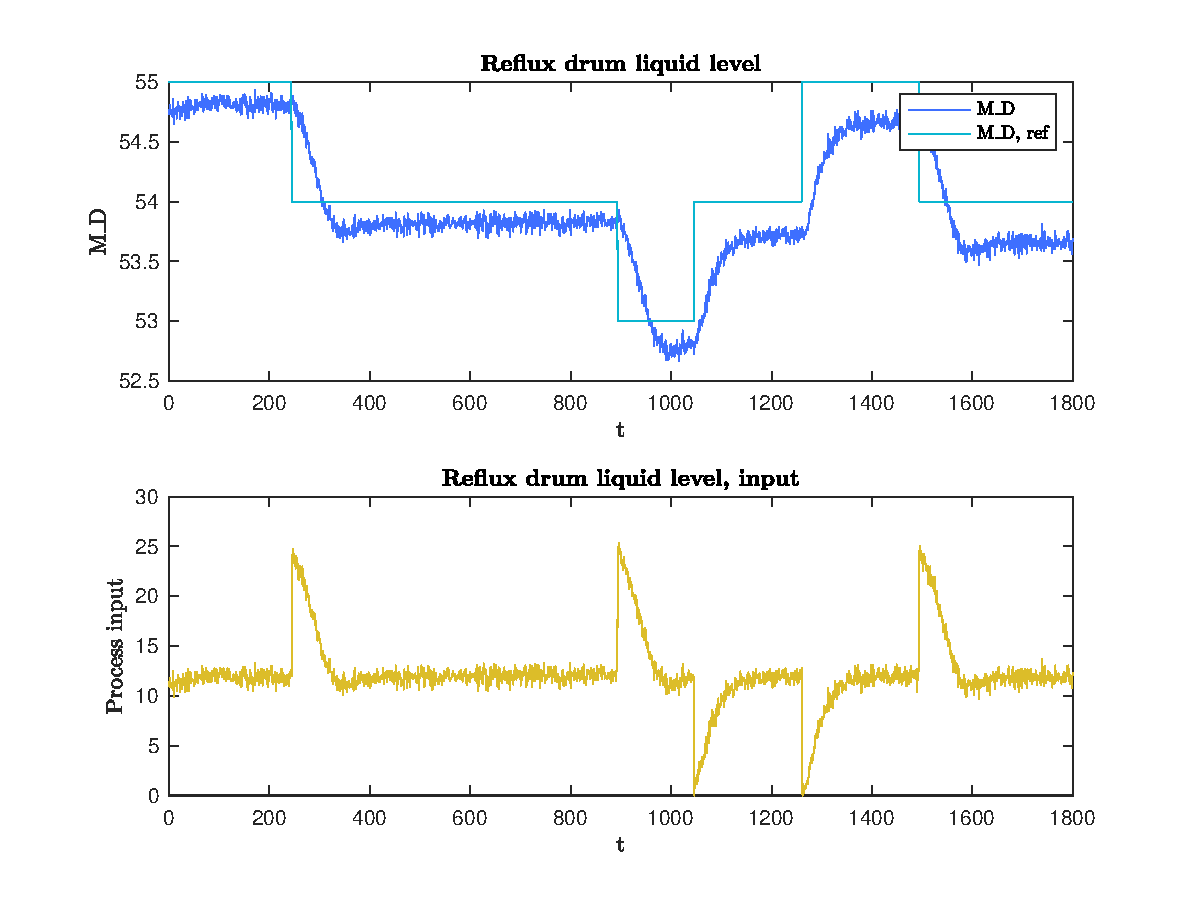
\includegraphics[width=0.8\textwidth]{../Systemanalyse/Log_Data_to_Matlab/Figurer/Identifisering/MD_eksperiment.eps}
\caption{System identification experiment for $M_D$ controller}
\label{fig:MD_experiment}

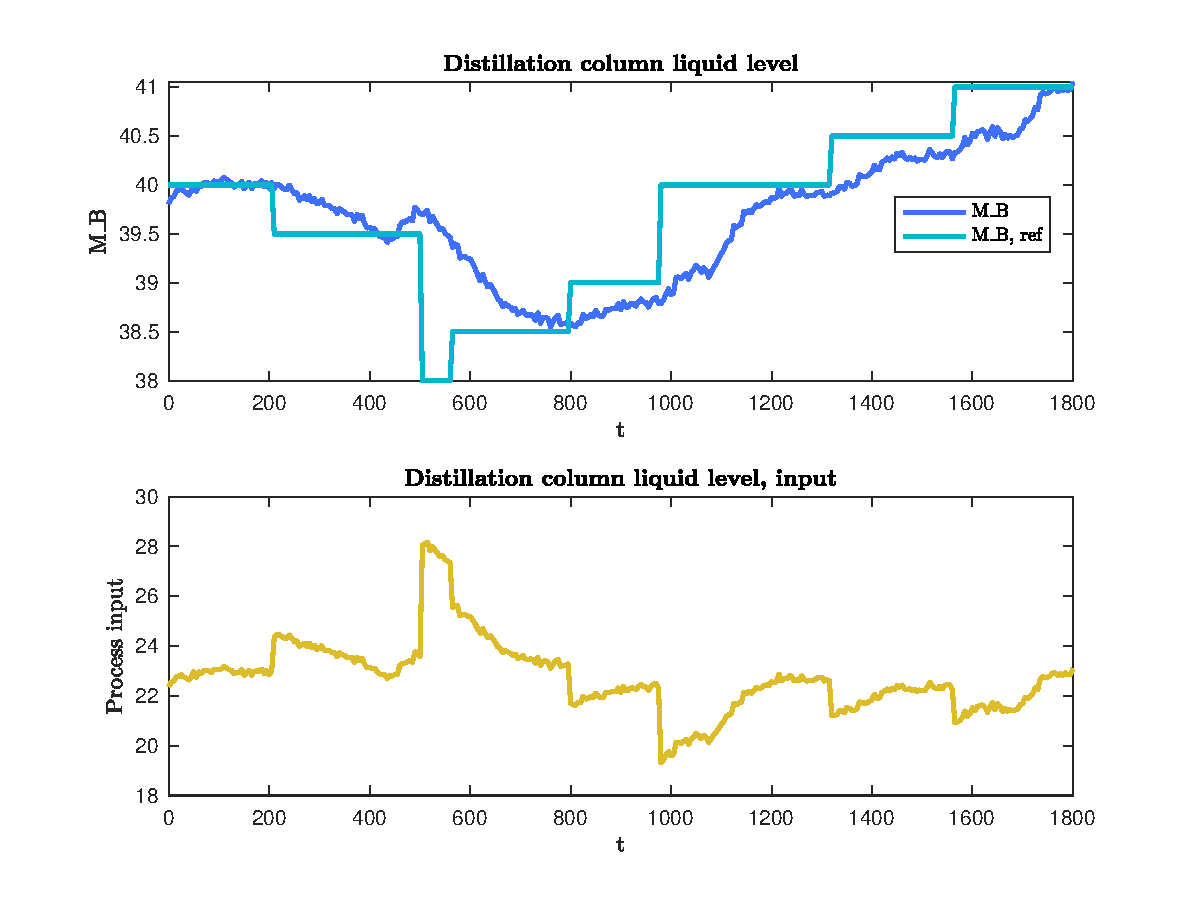
\includegraphics[width=0.8\textwidth]{../Systemanalyse/Log_Data_to_Matlab/Figurer/Identifisering/MB_eksperiment.eps}
\caption{System identification experiment for $M_B$ controller}
\label{fig:MD_experiment}
\end{figure}

\begin{figure}
\centering
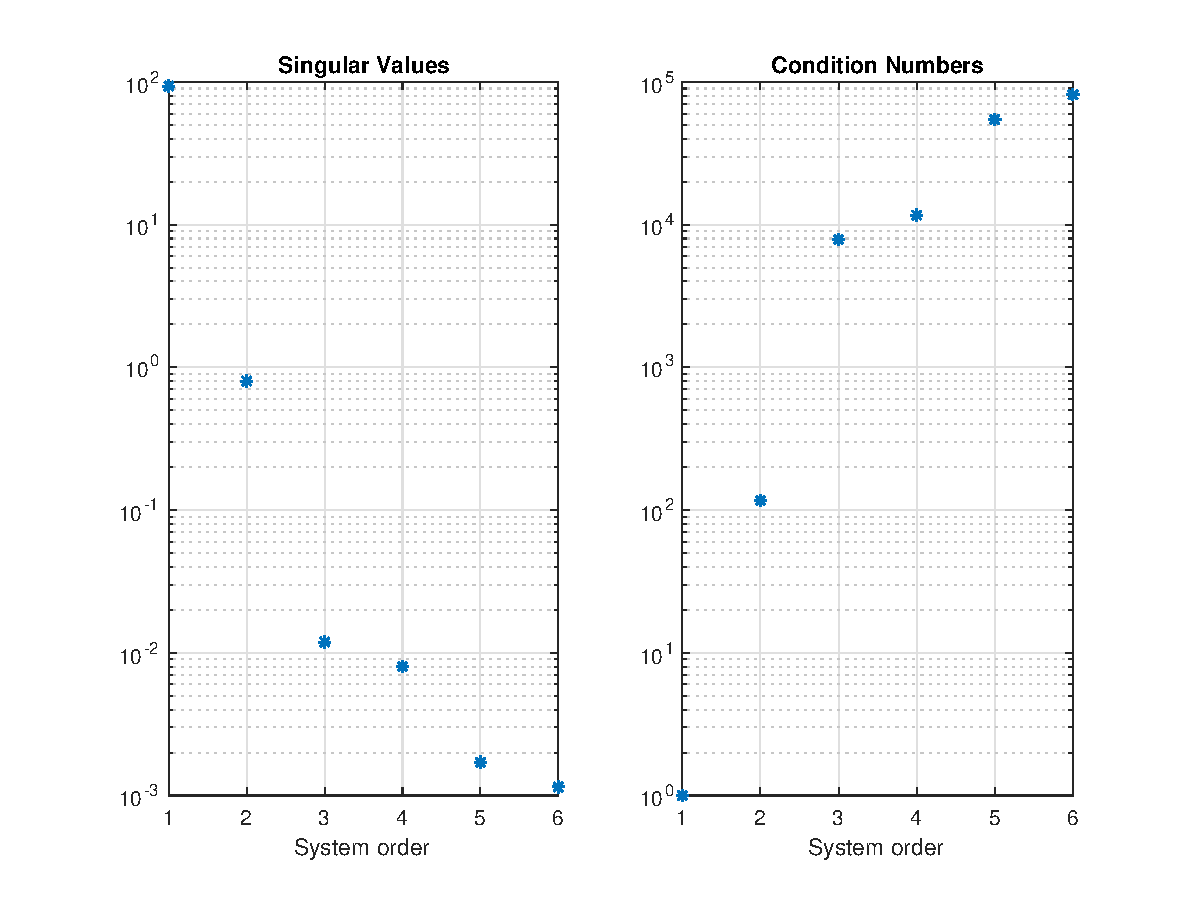
\includegraphics[width=0.8\textwidth]{../Systemanalyse/Log_Data_to_Matlab/Figurer/Identifisering/d-sr_info.eps}
\caption{Minimal singular value and condition number}
\label{fig:d-sr_info}
\end{figure}

\begin{figure}
\centering
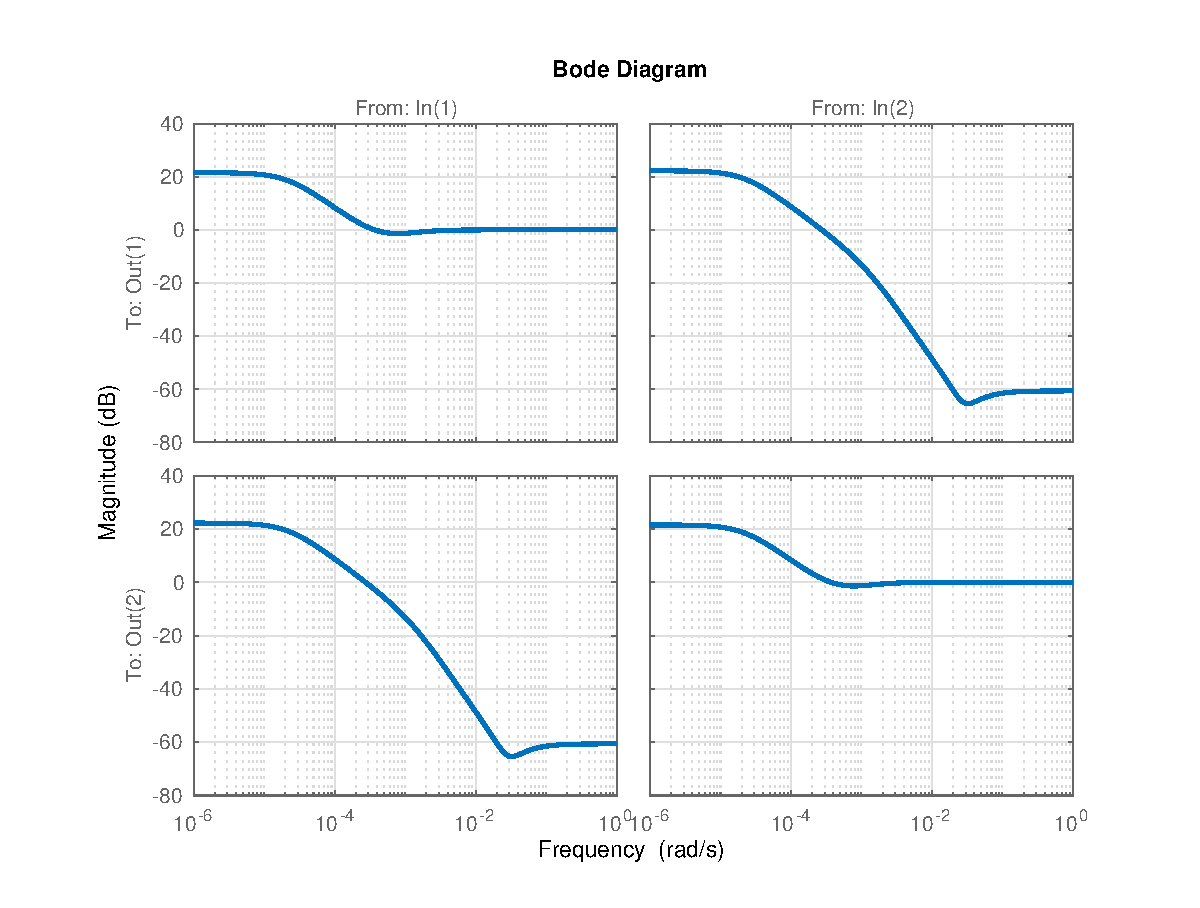
\includegraphics[width=0.8\textwidth]{../Systemanalyse/Log_Data_to_Matlab/Figurer/Identifisering/BD_RGA.eps}
\caption{Magnitude of RGA of identified system}
\label{fig:BD_RGA}
\end{figure}

\begin{figure}
\centering
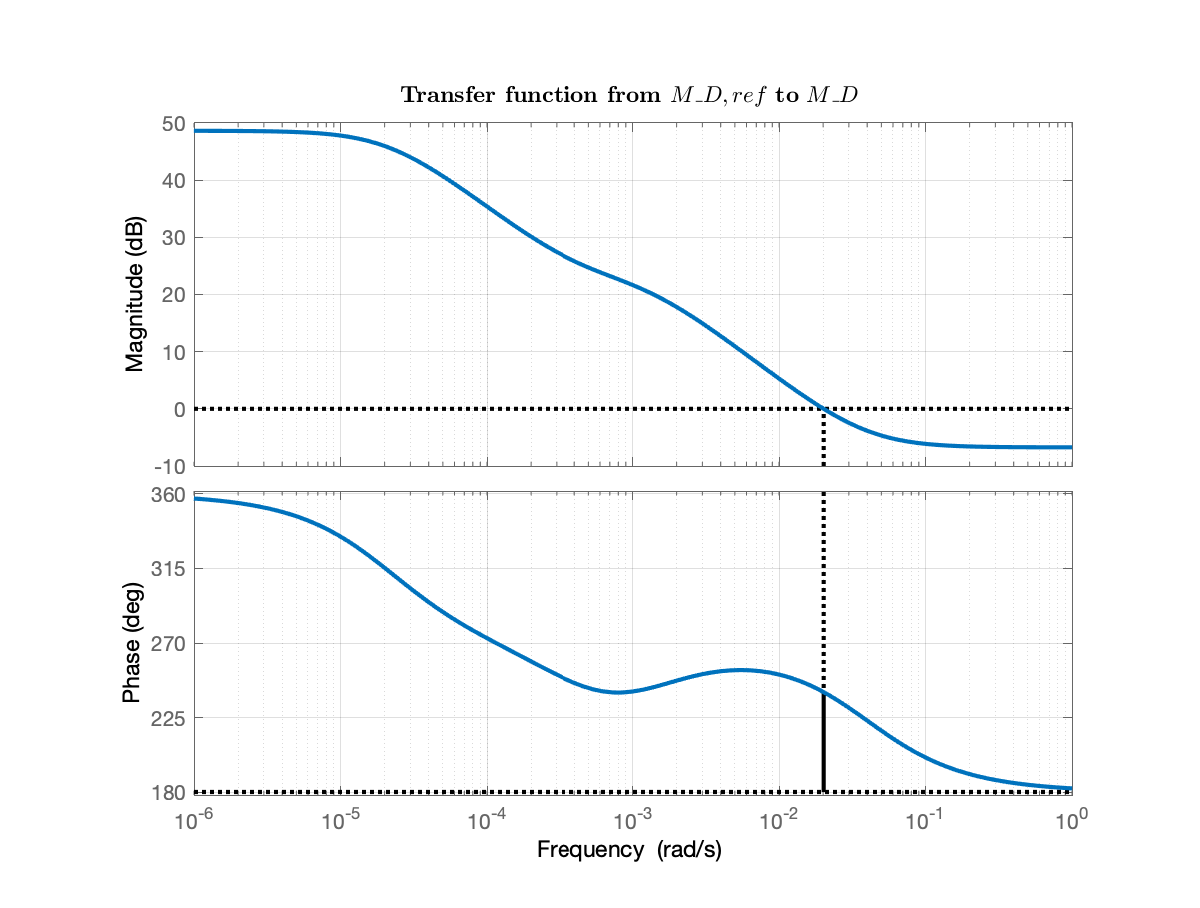
\includegraphics[width=0.8\textwidth]{../Systemanalyse/Log_Data_to_Matlab/Figurer/Identifisering/MD_bode.eps}
\caption{Magnitude and phase response of reflux drum level from reflux drum level reference}
\label{fig:L11}

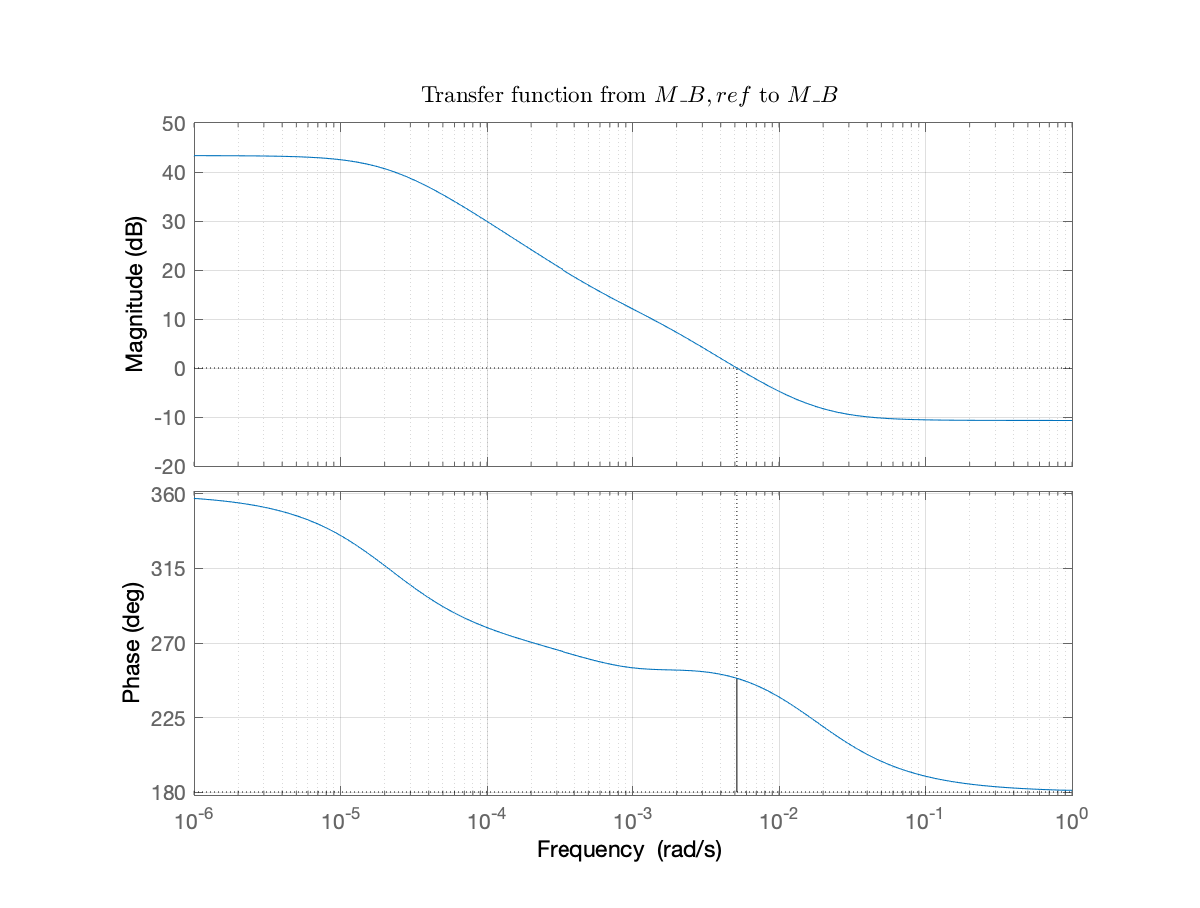
\includegraphics[width=0.8\textwidth]{../Systemanalyse/Log_Data_to_Matlab/Figurer/Identifisering/MB_bode.eps}
\caption{Magnitude and phase response of distillation column level from distillation column level reference}
\label{fig:L22}
\end{figure}

\todo{Dette er teknisk sett transferfunksjon fra feil til tilstand, ikke fra referanse}

\begin{figure}
\centering
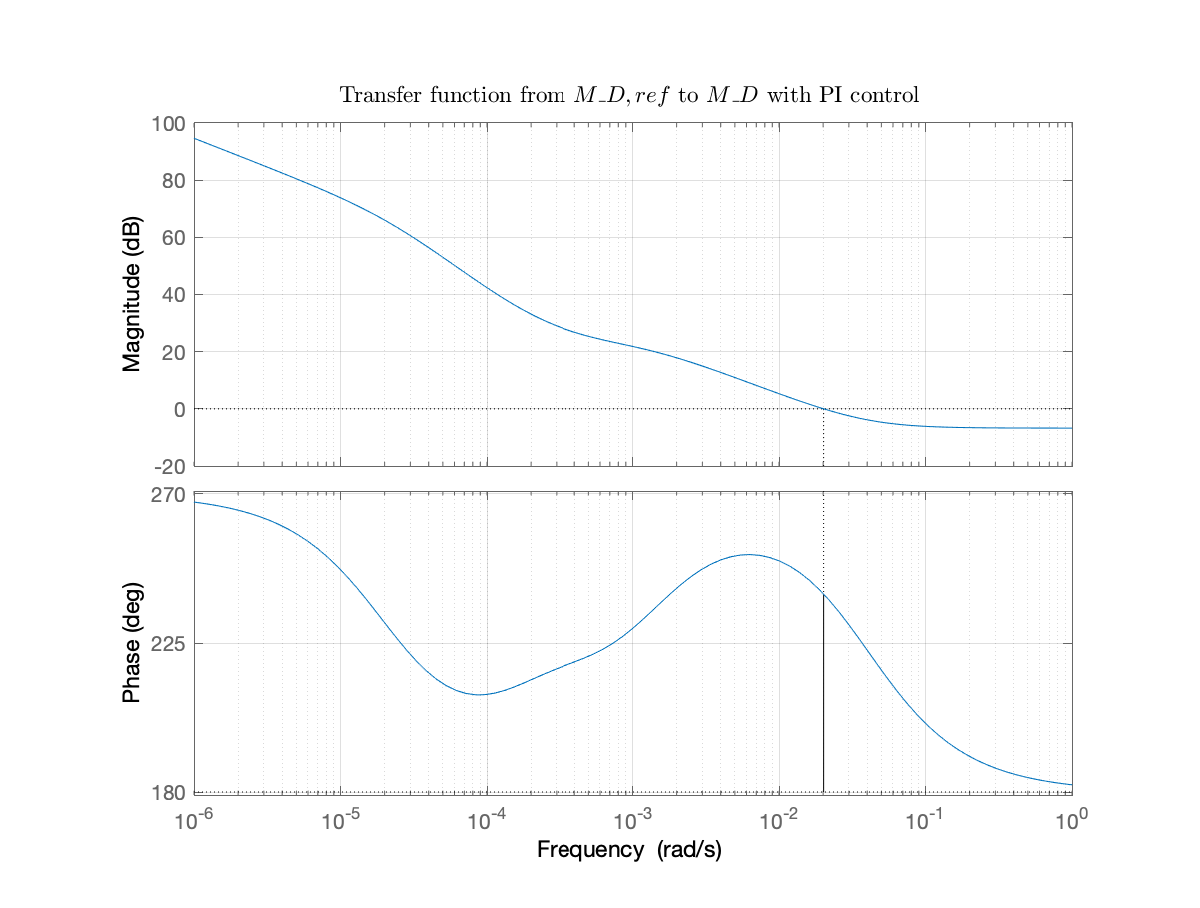
\includegraphics[width=0.8\textwidth]{../Systemanalyse/Log_Data_to_Matlab/Figurer/Identifisering/MD_PI_bode.eps}
\caption{Magnitude and phase response of reflux drum level from reflux drum level reference, using suggested PI controller}
\label{fig:L11_PI}

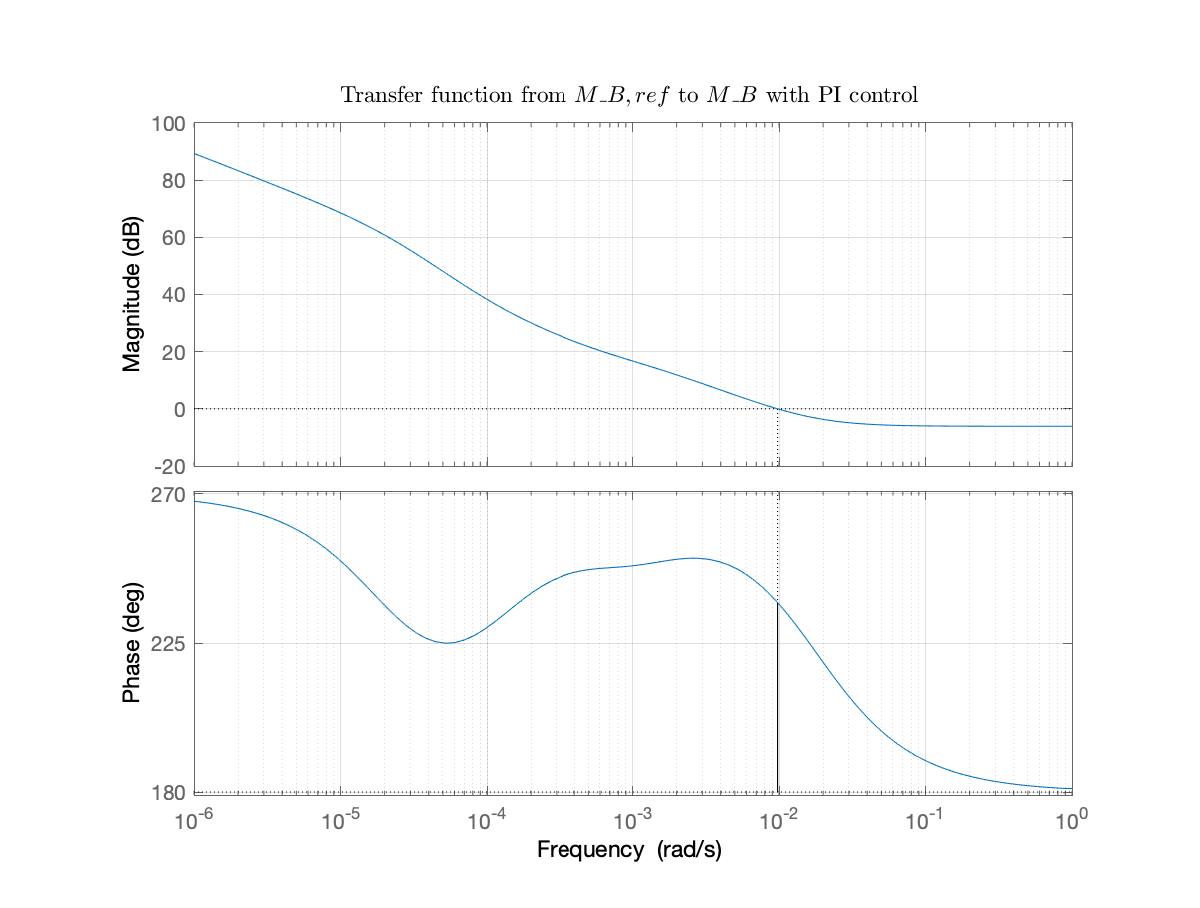
\includegraphics[width=0.8\textwidth]{../Systemanalyse/Log_Data_to_Matlab/Figurer/Identifisering/MB_PI_bode.eps}
\caption{Magnitude and phase response of distillation column level from distillation column level reference, using suggested PI controller}
\label{fig:L22_PI}
\end{figure}

\begin{figure}
\centering
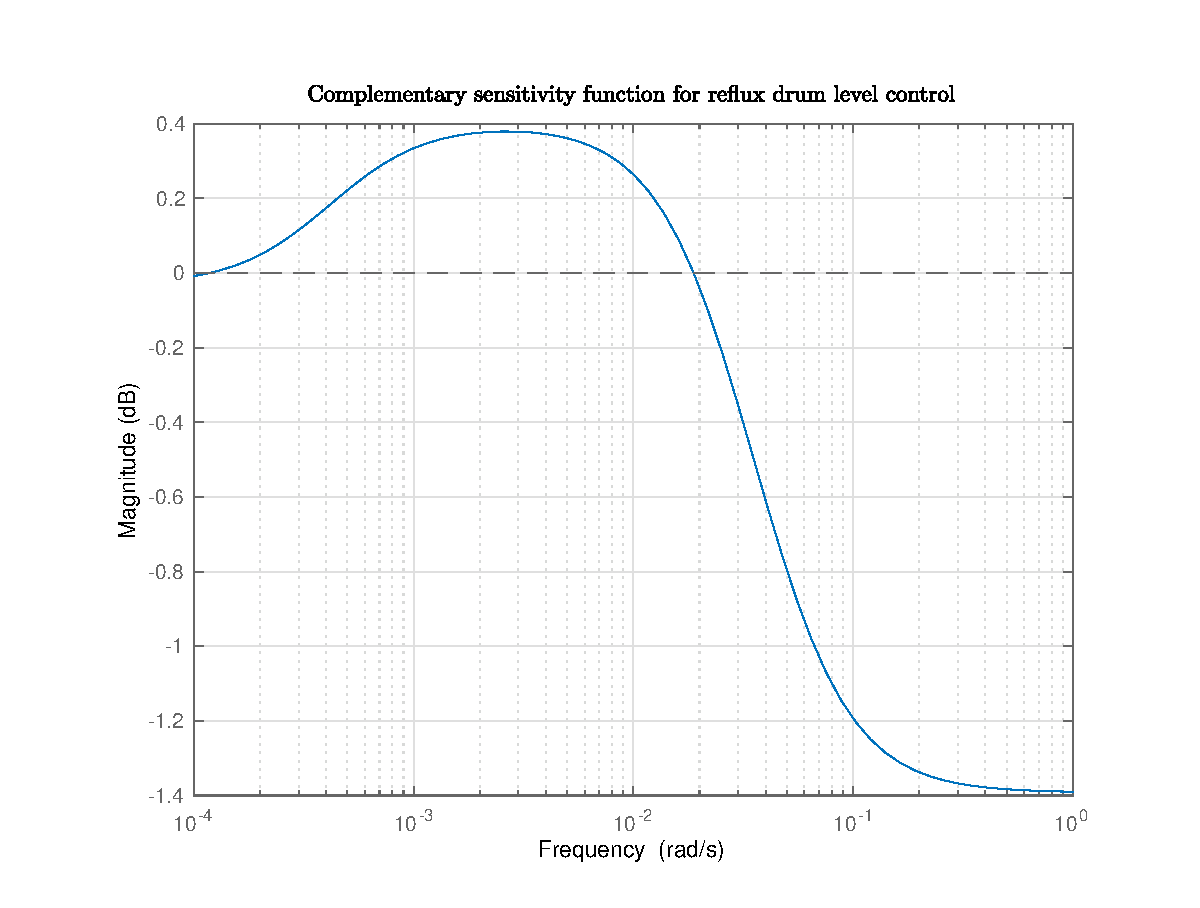
\includegraphics[width=0.8\textwidth]{../Systemanalyse/Log_Data_to_Matlab/Figurer/DB_tuning/T1.eps}
\caption{Complementary sensitivity function for reflux drum level control}
\label{fig:T1}

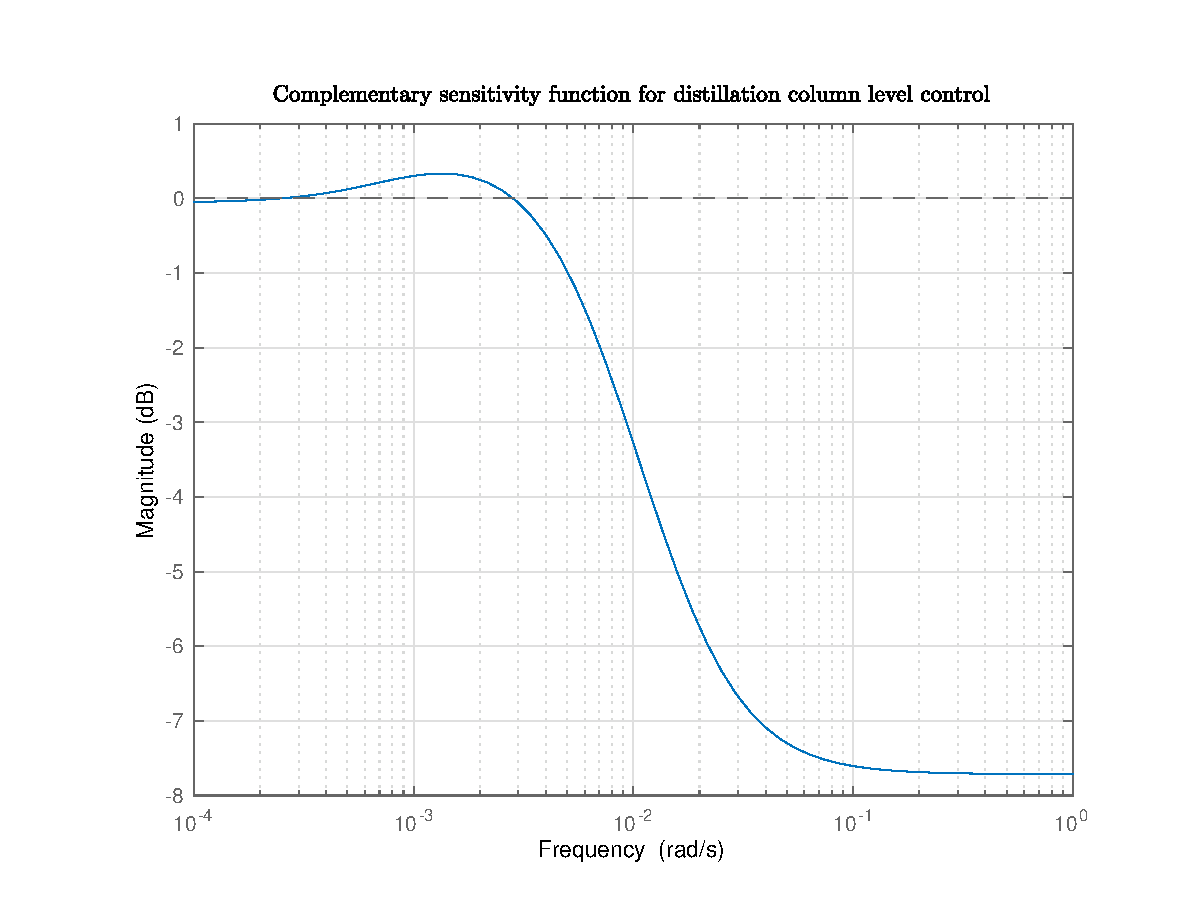
\includegraphics[width=0.8\textwidth]{../Systemanalyse/Log_Data_to_Matlab/Figurer/DB_tuning/T2.eps}
\caption{Complementary sensitivity function for distillation column level control}
\label{fig:T2}
\end{figure}

\subsection{Controller tuning}
Simulation in K-spice showed stationary deviation in $M_D$. To counteract this, the integral time was reduced. Control of $M_B$ worked satisfactory using the PI controller derived from the frequency analysis above.

The initial parameters based on loop-shaping, and the final ones are shown in table \ref{tab:DB_parameters}.

\begin{table}[h]
\centering
\begin{tabular}{c | c | c : c | c}
 & $K_{p, \textrm{initial}}$ & $T_{i, \textrm{initial}}$ & $K_{p, \textrm{final}}$ & $T_{i, \textrm{final}}$\\ \hline
 $M_D$ & 1200 & 5000s & 1200 & 1000s \\
 $M_B$ & 2000 & 5000s & 2000 & 5000s
\end{tabular}
\caption{Parameters for level controllers}
\label{tab:DB_parameters}
\end{table}

\todo{Simulate and plot step responses from K-spice}

\newpage
\section{Composition controllers}
Let $y = [T_D \quad T_B]^T$, $r = [T_{D, \textrm{ref}} \quad T_{B, \textrm{ref}}]^T$ and $u = [L \quad V]^T$. By changing the setpoints for the manipulated variables $L$ and $V$, the system transfer function
\begin{equation}
G(s) = \frac{y}{u}(s)
\end{equation}
may be identified directly.
\subsection{System identification and analysis}
\subsubsection{Experiment}
Identification of the LV system was done in a similar manner as in the previous section, using step changes in input (but open-loop this time). Again, \texttt{d-sr} was used for identification. 

\todo[inline]{Gjennomfør eksperiment}

\subsubsection{Analysis}
\todo[inline]{Presenter relevant teori}

\subsection{Controller tuning}
\todo[inline]{Tune i K-spice}


\newpage
\section{Results}
\subsection{PI controller tuning}
Table \ref{tab:final_controller_parameters} shows the final PI controller parameters for all the control loops tuned in this project, also including the scaled gain $G$ used in the K-spice implementation.

\begin{table}
\centering
\begin{tabular}{c | c | c | c }
& $K_p$ & $G$ & $T_i$ \\ \hline
$D$ (FC1005) & 0,0035 & 0,42& 0,4s\\
$L$ (FC1015) & 0,0018 & 0,22 & 1,0s \\
$B$ (FC1019) & 0,0025 & 0,3 & 1,0s \\
$V$ (LC1028) & 200 & 200 & 10s \\
$p$ (PC1024) & 5 & 30 & 20s \\
$M_D$ (LC1016) & 1200 & 10 & 1000s \\
$M_B$ (LC1015) & 2000 & 16,7 & 5000s \\
$T_D$ (TC1015) & 12 & 2,5 & 100s \\
$T_B$ (TC1088) & 30 & 6,3 & 1000s
\end{tabular}
\end{table}

\subsection{Reference tracking}
The results of step changes in reference are shown in figures \ref{fig:T_D_step} and \ref{fig:T_B_step}.

\begin{figure}
\centering
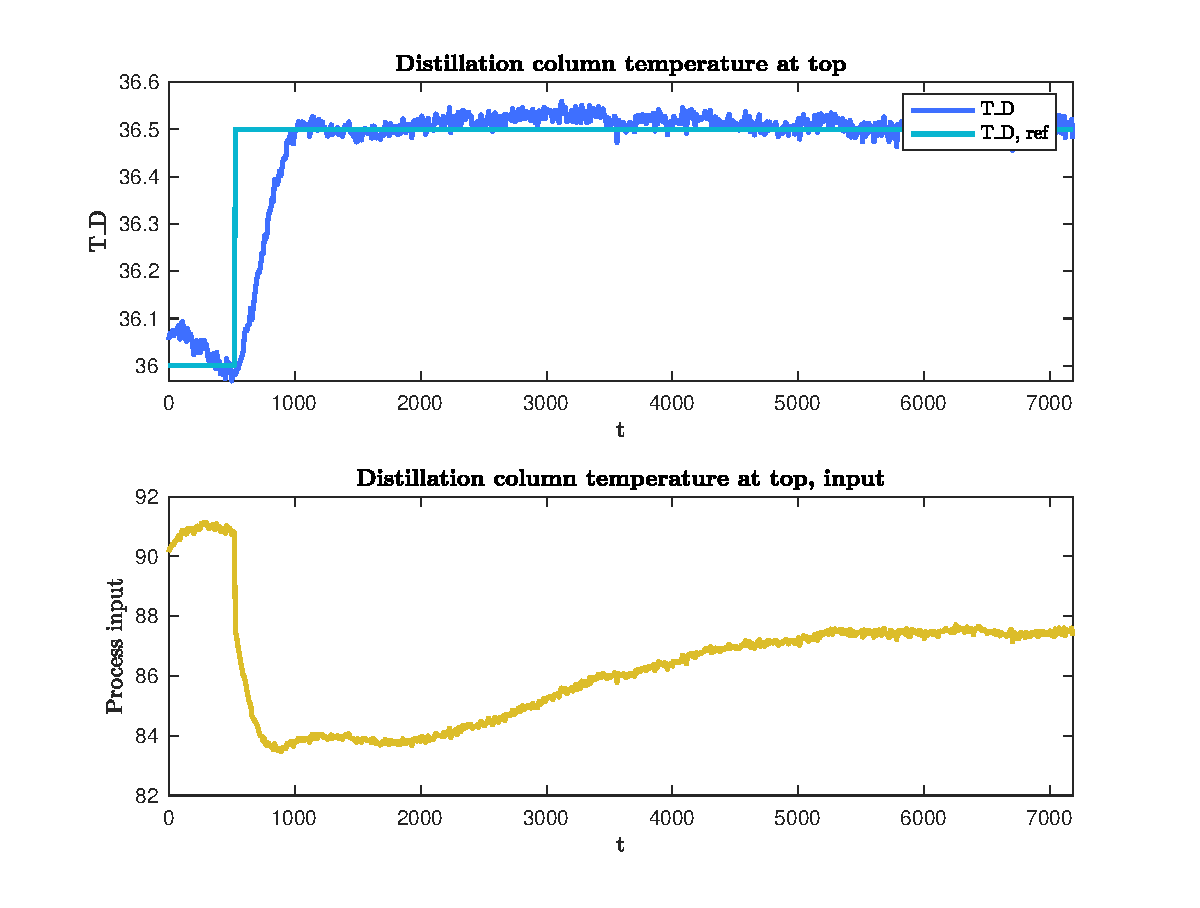
\includegraphics[width=0.8\textwidth]{../Systemanalyse/Log_Data_to_Matlab/Figurer/LV_tuning/T_D_with_T_D_step.eps}
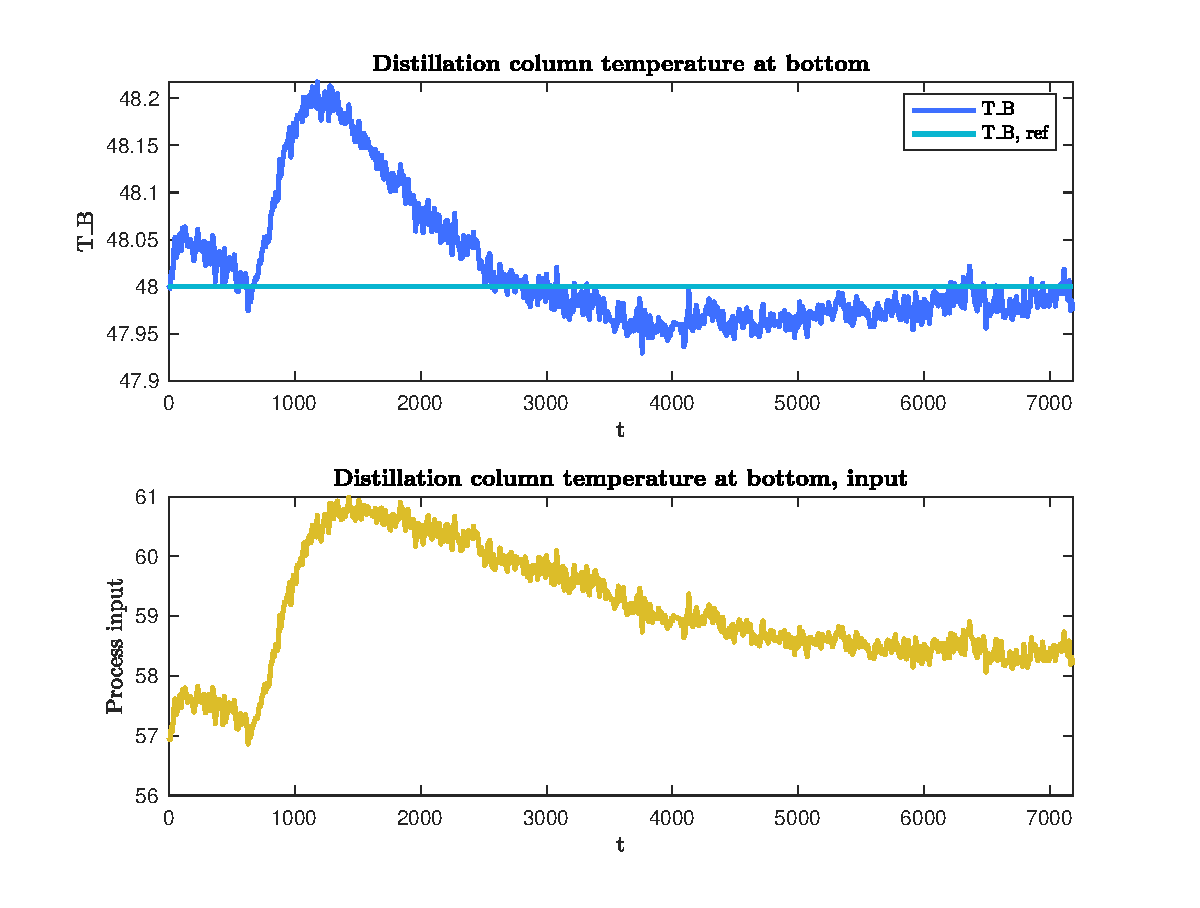
\includegraphics[width=0.8\textwidth]{../Systemanalyse/Log_Data_to_Matlab/Figurer/LV_tuning/T_B_with_T_D_step.eps}
\caption{Response of $T_D$ and $T_B $ to step change in $T_{D, \textrm{ref}}$}
\label{fig:T_D_step}
\end{figure}

\begin{figure}
\centering
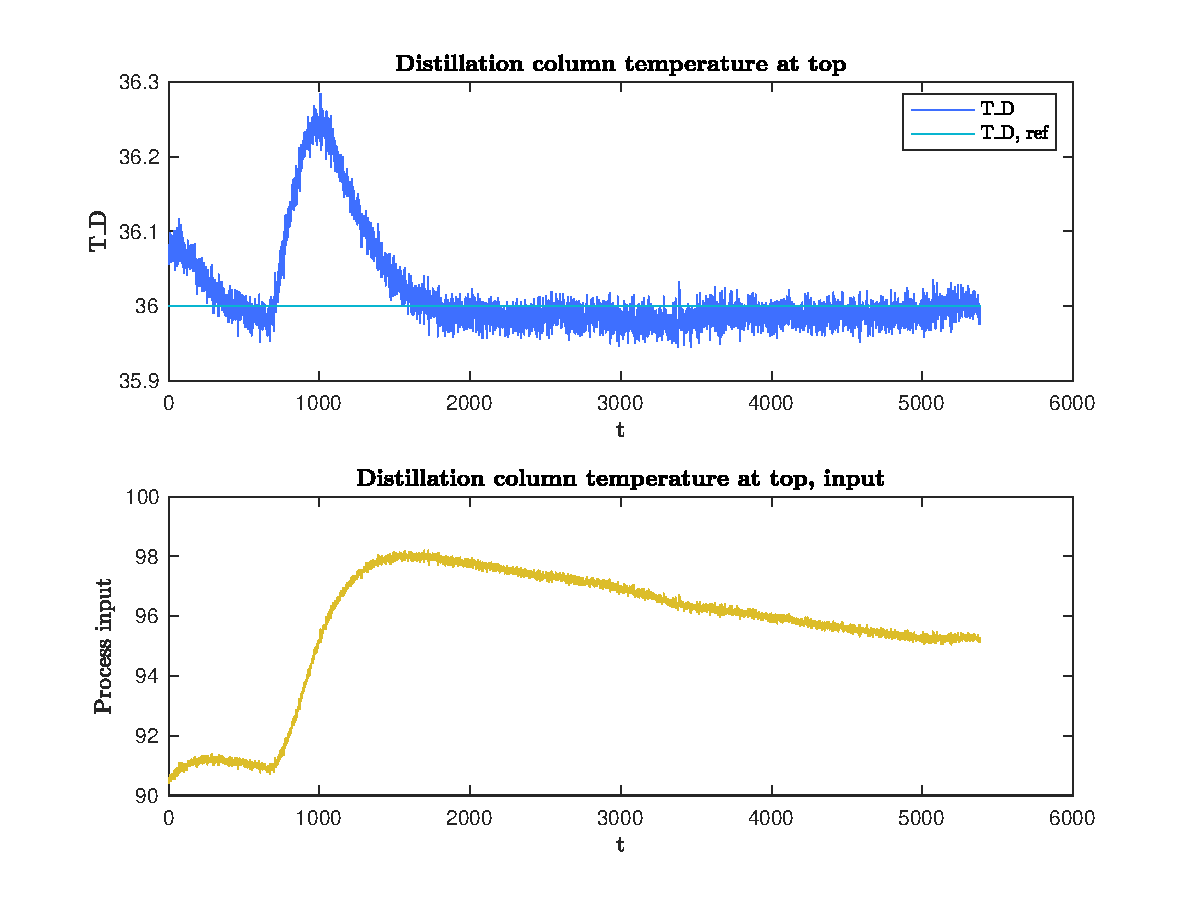
\includegraphics[width=0.8\textwidth]{../Systemanalyse/Log_Data_to_Matlab/Figurer/LV_tuning/T_D_with_T_B_step.eps}
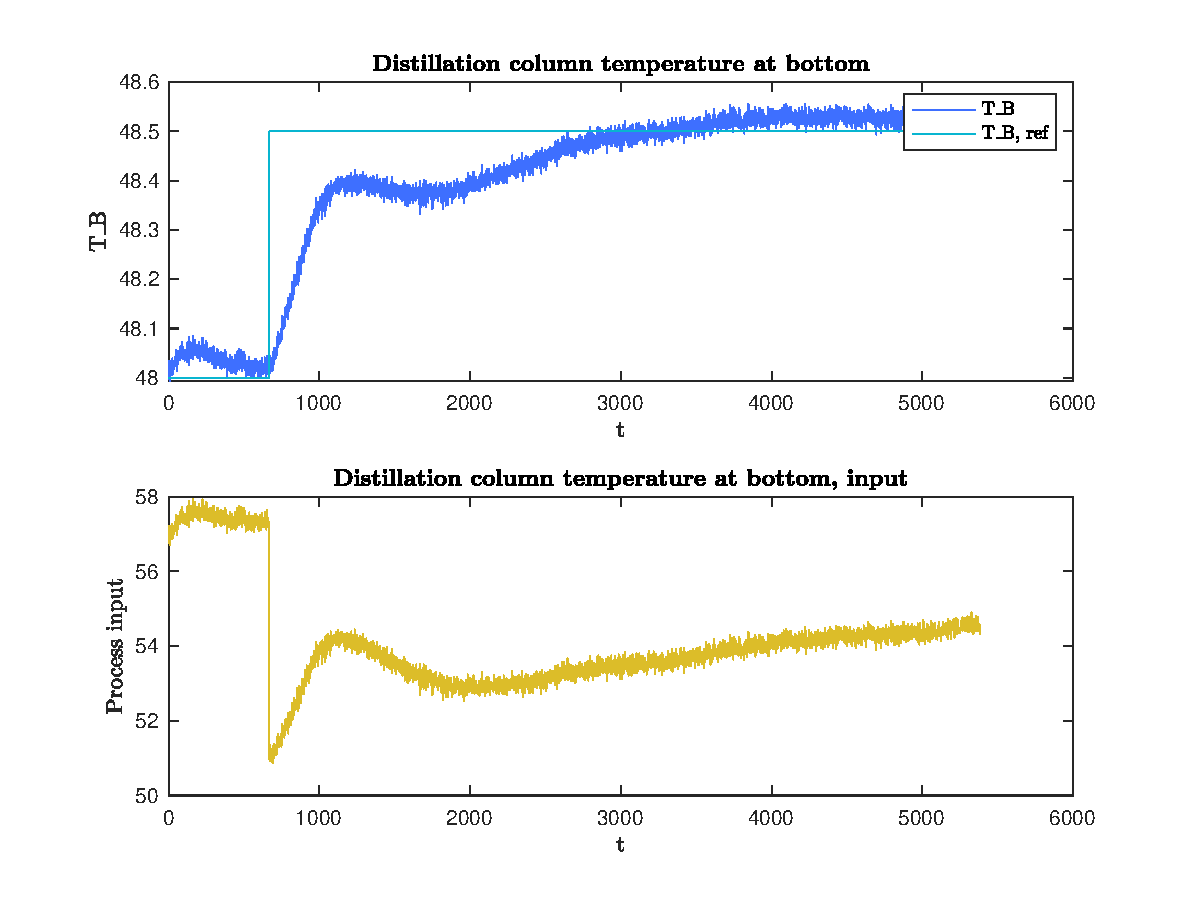
\includegraphics[width=0.8\textwidth]{../Systemanalyse/Log_Data_to_Matlab/Figurer/LV_tuning/T_B_with_T_B_step.eps}
\caption{Response of $T_D$ and $T_B $ to step change in $T_{B, \textrm{ref}}$}
\label{fig:T_B_step}
\end{figure}

\end{document}
